\chapter{Software}

O subsistema de software do projeto é parte fundamental do projeto por proporcionar a interação entre o usuário e o radar. Para explicar a estrutura e funcionamento, falaremos dos requisitos, casos de uso, microsserviços, banco de dados, resiliência na comunicação do software, comunicação entre software e eletrônica e representação arquitetural dele. Além disso, apresentaremos protótipos para deixar mais claro como será a interface de usuário.

\section{Requisitos}

Para a construção dos produtos de software, a equipe do projeto RaDop levantou -- por meio da técnica \textit{brainstorming} (elicitação com os membros do projeto e reuniões presenciais) -- os requisitos que guiarão o desenvolvimento das soluções para o radar.

Os requisitos estão dividos por sistemas de software, sendo eles o aplicativo da manutenção (de nome RaDop) e o \textit{WebApp} do \textit{Dashboard}. Também estão englobados requisitos que serão transformados em microsserviços específicos para o funcionamento do radar.

\subsection{Aplicativo RaDop}

Abaixo estão listados os requisitos funcionais e não funcionais do aplicativo móvel que será usado pela equipe de manutenção do RaDop. Começando pelos requisitos funcionais temos:


\begin{itemize}
  \item O aplicativo da manutenção deve receber dados do radar. Esses dados são:
  \begin{enumerate}
    \item Informação de calibração DC\footnote{Integração com a \textit{BladeRF} para calibração de parâmetros de funcionamento da placa, os sistemas de calibração serão produzidos pela equipe de eletrônica do projeto RaDop.};
    \item Operacionalidade: câmera, radiofrequência (Doppler) e \textit{Raspberry};
    \item Temperatura do equipamento;
    \item Nível de carga da bateria;
    \item Relatório de operação com falhas ocorridas em virtude de algum equipamento eletrônico apresentar problemas de funcionamento;
    \item Funcionamento do radar.
  \end{enumerate}
\end{itemize}

\begin{itemize}
    \item O aplicativo deve enviar notificações para o usuário nos seguintes casos:
    \begin{enumerate}
        \item Quando a carga da bateria estiver igual ou menor que 20\%;
        \item Em caso de falha de comunicação do aplicativo com o radar.
    \end{enumerate}
\end{itemize}


\begin{itemize}
    \item O aplicativo deve ter um registro de manutenção (\textit{CRUD}\footnote{\textit{CRUD}: Sigla em inglês para \textit{Create}, \textit{Read}, \textit{Update} e \textit{Delete}. Se trata do gerenciamento do objeto.}), anotando a data e o hórario de acesso ao radar, além do usuário que acessou.
\end{itemize}

\begin{itemize}
    \item O aplicativo deve ter um sistema de usuários (\textit{CRUD}) para identificação, cadastro e gerenciamento dos usuários do aplicativo.
    \item O aplicativo deve ter a capacidade de calibrar o radar a fim de auxiliar na manutenção corretiva do radar.
\end{itemize}

Os requisitos não funcionais do aplicativo do RaDop são:

\begin{itemize}
    \item O aplicativo deve ter acesso à internet para funcionar;
    \item O aplicativo deve ter um banco de dados para armazenar os dados e as manutenções;
    \item O radar não deve permitir que pessoas sem autorização o acesse;
    \item O usuário deve ter um aparelho com o sistema operacional Android para usar a aplicação (versão mínima: 5);
    \item A interface de usuário deve ter usabilidade e ser amigável;
    \item Deve haver um banco de dados para as informações do aplicativo.
\end{itemize}

\subsection{\textit{WebApp Dashboard}}

Abaixo estão listados os requisitos funcionais e não funcionais do \textit{WebApp Dashboard} do RaDop (voltado para equipes gestora dos radares).

\begin{itemize}
    \item O \textit{Dashboard} deve receber dados do radar. Esses dados são:
    \begin{enumerate}
        \item Quantidade de carros fotografados;
        \item Fotos tiradas dos carros;
        \item Quantidade de veículos acima da velocidade máxima e a velocidade deles no momento do flagrante;
        \item Data e horário das capturas;
        \item Notificações de automóveis flagrados;
        \item Notificações de possível acidente;
        \item Identificação do equipamento que enviou os dados.
    \end{enumerate}
\end{itemize}

\begin{itemize}
    \item O \textit{Dashboard} deve possibilitar a visualização dos dados enviados (gráficos e tabelas).
\end{itemize}

\begin{itemize}
    \item O \textit{Dashboard} deve recuperar os seguintes dados, a partir da placa do veículo:
    \begin{enumerate}
        \item Situação do carro (roubado/sem restrição);
        \item Cor;
        \item Ano;
        \item Marca;
        \item Modelo;
        \item Registro.
    \end{enumerate}
\end{itemize}

\begin{itemize}
    \item O \textit{Dashboard} deve possibilitar obter informações complementares a partir dos dados recebidos para realizar \textit{data mining}\footnote{Data Mining: A partir dos dados recebidos extrair dados terciários a fim de obter novos conhecimentos, identificar padrões, relacionamentos sistemáticos e etc.}.
    \item O \textit{Dashboard} deve exibir a localização dos radares (mapa);
    \item O \textit{Dashboard} deve ter um sistema de usuários (\textit{CRUD});
    \item O \textit{Dashboard} deve ter um sistema de visualização/notificação de veículos irregulares;
    \item O \textit{Dashboard} deve ter um sistema de visualização/notificação de acidentes;
    \item O aplicativo deve ter a capacidade de calibrar o radar a fim de auxiliar na manutenção corretiva do radar.
\end{itemize}

Os requisitos não funcionais são:

\begin{itemize}
    \item O \textit{Dashboard} deve manter comunicação com os microsserviços;
    \item O \textit{Dashboard} deve ter de um banco de dados para armazenar os dados e as manutenções;
    \item O \textit{Dashboard} não deve permitir que pessoas sem a autorização correta o acesse;
    \item A interface de usuário deve ter usabilidade e ser amigável;
    \item O \textit{Dashboard} deve ter um banco de dados para armazenar as suas informações.
\end{itemize}

\section{Casos de Uso}

O diagrama de casos de uso tem como objetivo documentar o que o sistema faz do ponto de vista do usuário. Em outras palavras, ele descreve as principais funcionalidades do sistema e a interação dessas funcionalidades com os usuários do mesmo. Nesse diagrama não haverá aprofundamento dos detalhes técnicos que dizem como o sistema faz.

Segue abaixo os diagramas de casos de uso do Aplicativo e do \textit{Dashboard}.

\begin{figure}[ht]
	\center{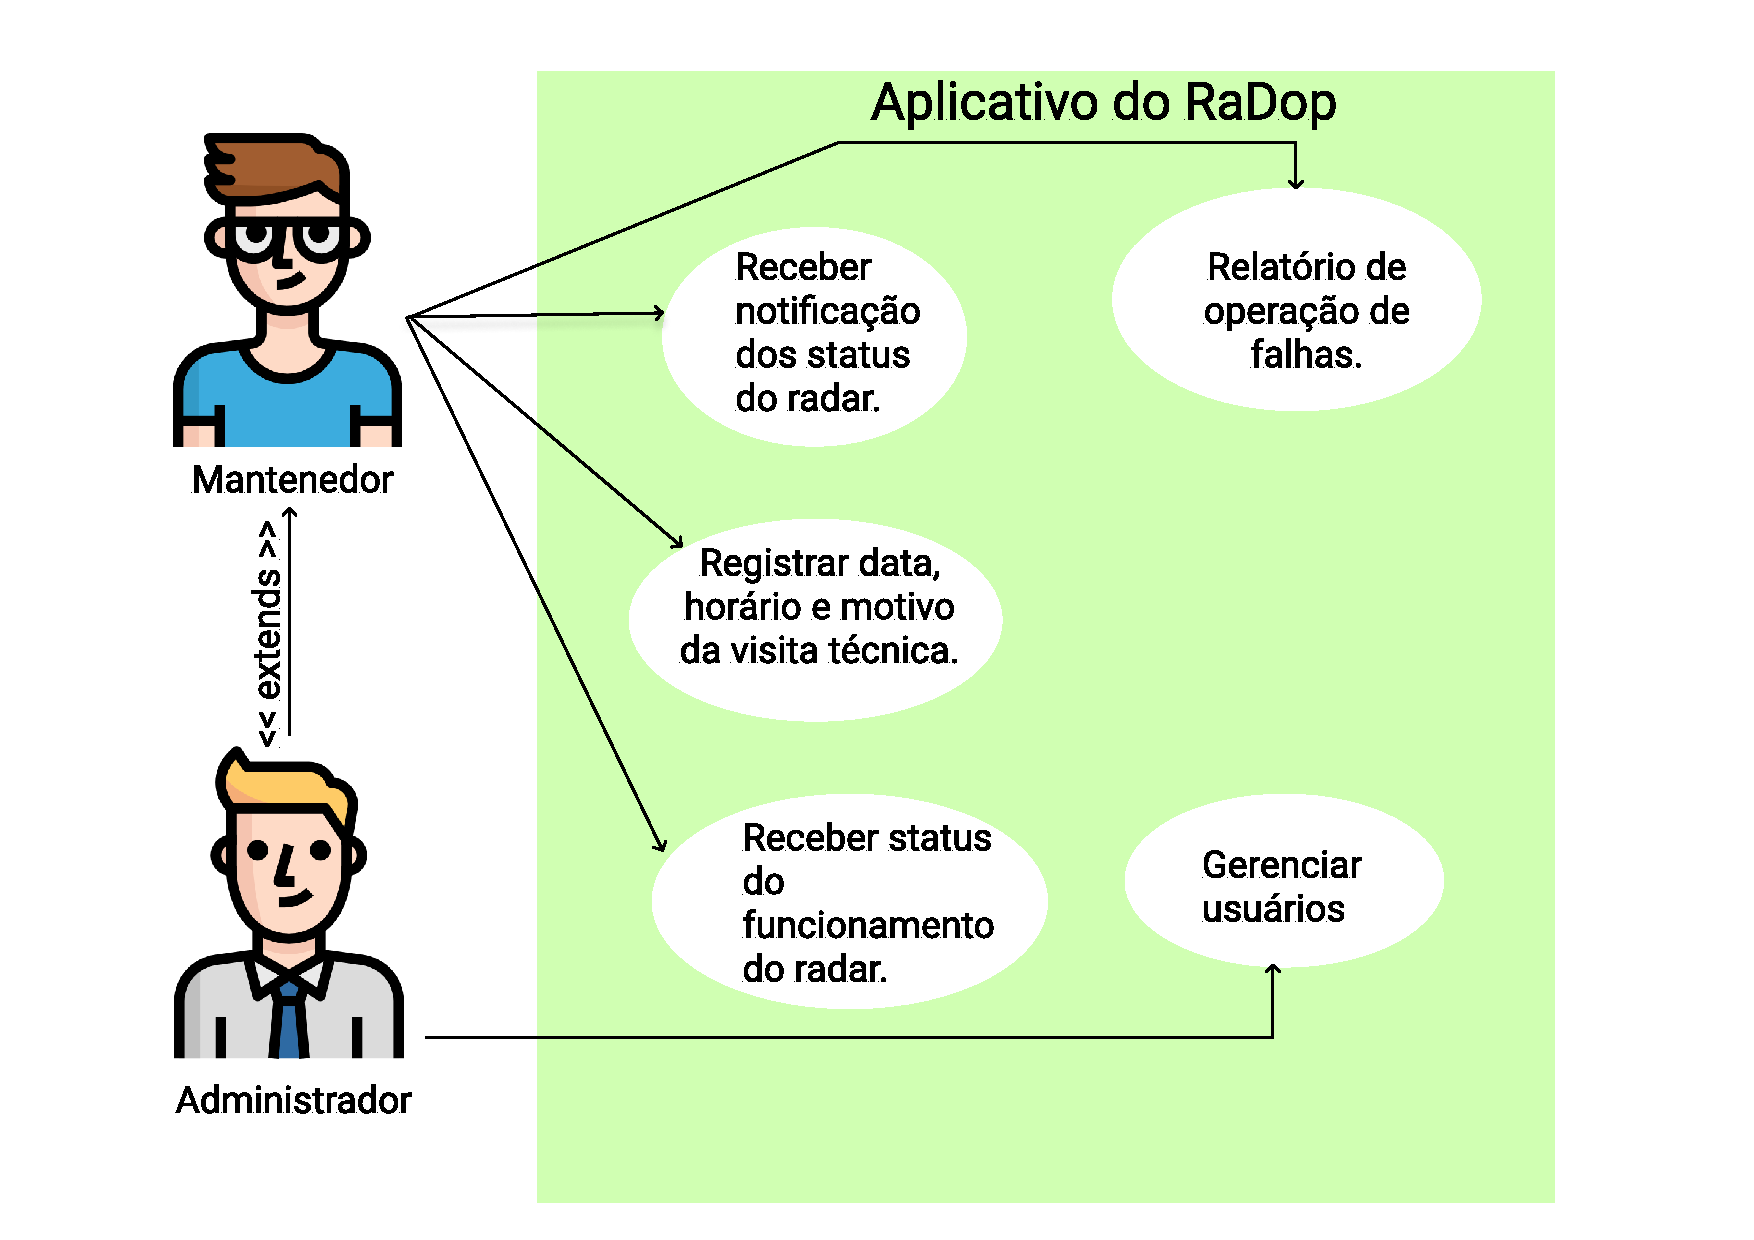
\includegraphics[scale=0.5]{caso_de_uso_app.pdf}}
	\caption{\label{fig:casos_de_uso} Diagrama de casos de uso com as principais funcionalidades do aplicativo RaDop.}
\end{figure}\newpage

\begin{figure}[ht]
	\center{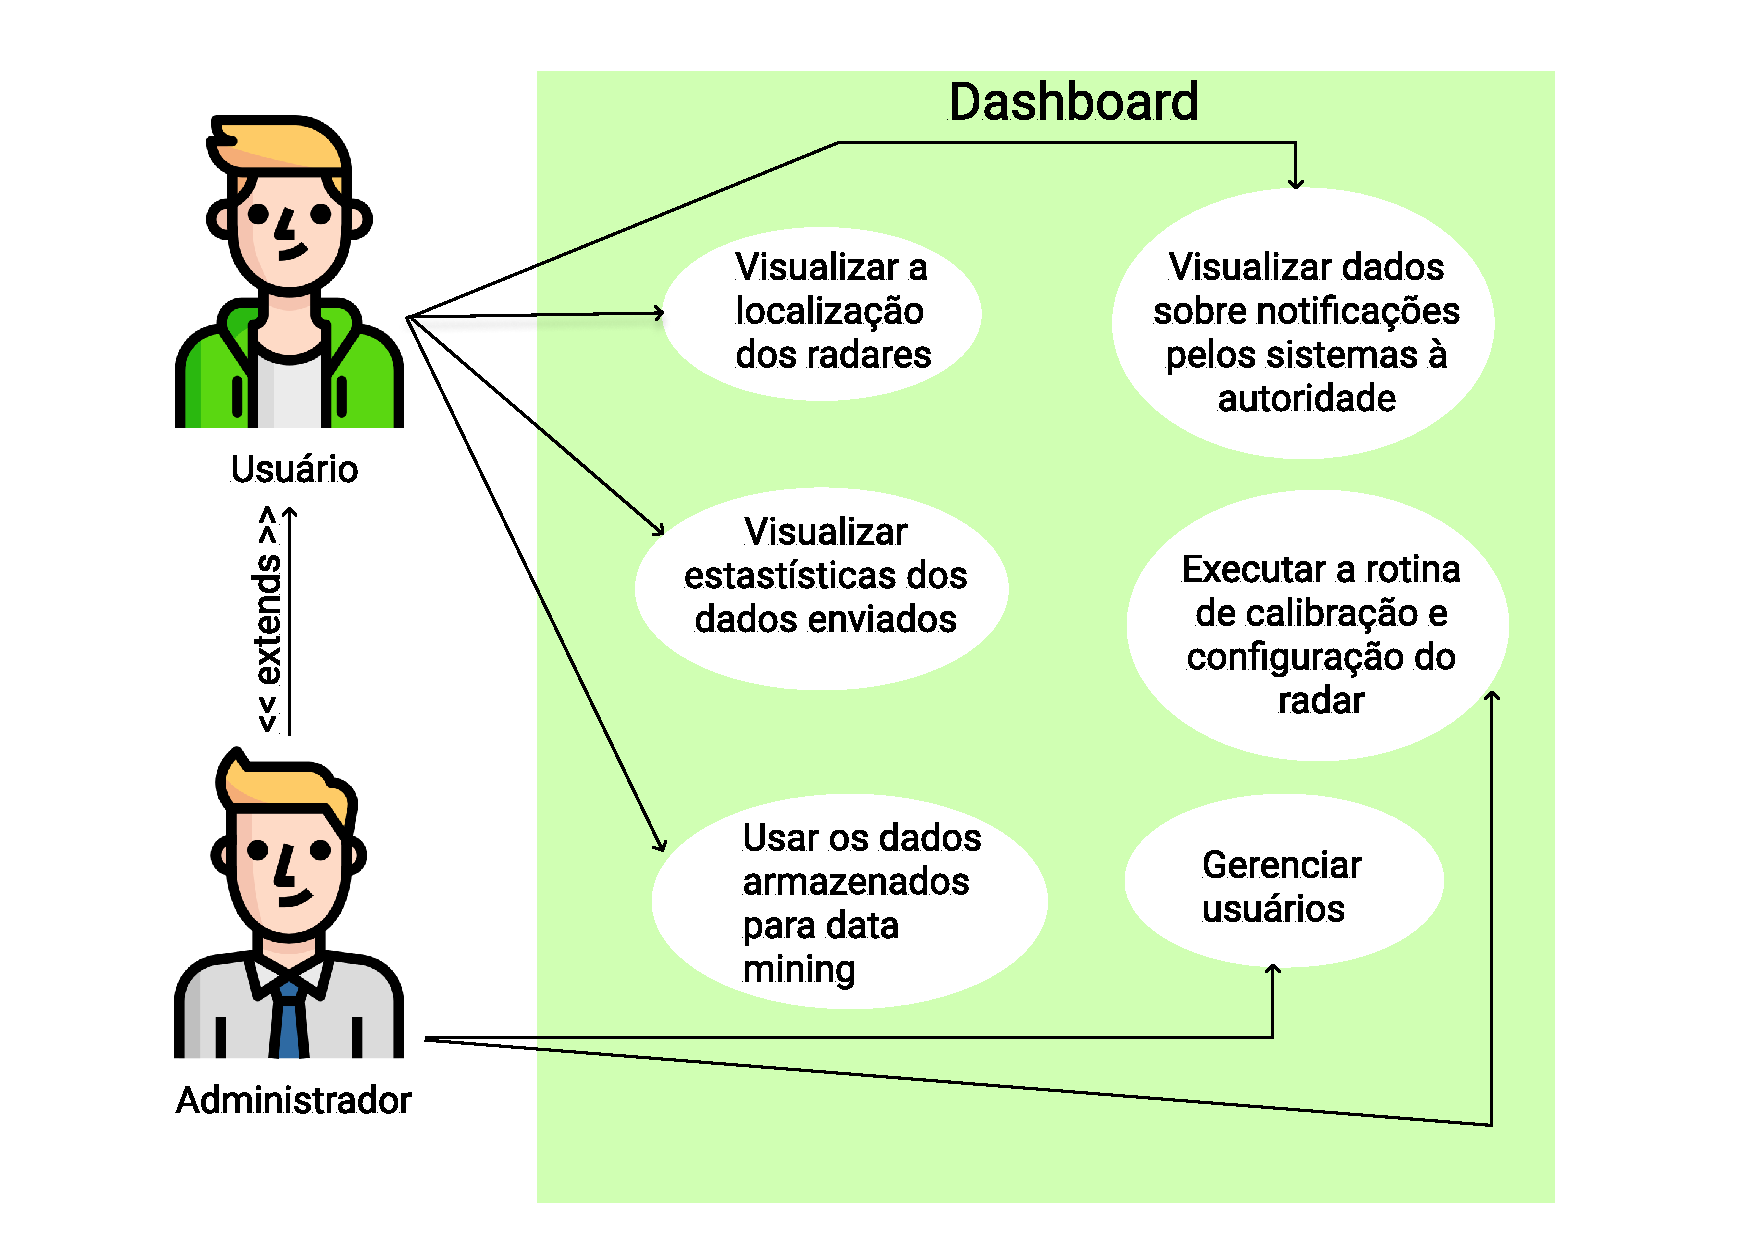
\includegraphics[scale=0.5]{caso_de_uso_dashboard.pdf}}
	\caption{\label{fig:diagrama-comm-soft} Diagrama de casos de uso com as principais funcionalidades do \textit{Dashboard}.}
\end{figure}

\section{\textit{Dashboard}}

A arquitetura do \textit{Dashboard}, esquematizada na Figura \ref{fig:diagrama-arq-dashboard}, será principalmente a baseada em componentes. O motivo para isso se deve ao uso do \textit{Django Application} do \textit{framework Django}, que é a principal tecnologia que será usada com o \textit{Dashboard}.

O uso de componentes permite uma série de vantagens. A primeira é construir componentes com alta coesão e baixo acoplamento, o que melhora a manutenibilidade do código. Outra é que eles podem ser totalmente independentes entre si. As vantangens citadas acabam permitindo que componentes criados possam ser reaproveitados em vários projetos, evitando retrabalho desnecessário e assim otimizando o tempo dos desenvolvedores envolvidos no projeto.

Uma tecnologia importante que também será utilizada em conjunto com o \textit{Dashboard} é o NGINX. Ele será utilizado para fazer o proxy reverso da aplicação. De modo resumido, ele vai atuar como uma espécie de organizador, redirecionando as requisições que chegam dos clientes para os contêineres corretos.

\section{Aplicativo RaDop}

Conforme mostra a Figura \ref{fig:diagrama-arq-webApp}, o applicativo móvel que irá auxiliar a equipe de manutenção não irá acessar o radar diretamente, mas sim através dos microsserviços. Deste modo, os microsserviços funcionarão como uma espécie de interface entre o radar e o aplicativo.

\section{Microsserviços}

Conforme definido na fase de iniciação de projeto do radar RaDop, e anteriormente citado, além do aplicativo e do \textit{WebApp} de \textit{Dashboard}, alguns dos outros serviços de software serão montados no formato de microsserviços, cuja arquitetura está esquematizada na Figura \ref{fig:diagrama-arq-microsservicos}.

Logo, a partir da elicitação dos requisitos, tanto do projeto quanto dos outros produtos de software, a equipe levantou quais são os microsserviços que devem ser construídos. Lembrando que microsserviço é uma abordagem para desenvolver uma única aplicação como uma suíte de serviços, cada um rodando em seu próprio processo e se comunicando entre eles através de mecanismos leves. Segundo Fowler e Lewis \cite{fowler2015}, estes serviços são construídos através de pequenas responsabilidades e publicados em produção de maneira independente.

Alguns dos microsserviços serão produzidos no formato de \textit{FaaS} (\textit{Function as a Service}), função como serviço, segundo Freitas \cite{freitas2018} estas funções são um serviço de computação em nuvem que busca abstrair a questão de servidor e máquinas onde rodam os seus programas. Em detalhes, ela deriva da filosofia \textit{Servless}, que delega ao provedor de computação em nuvem (\textit{Cloud Provider}) provisionar uma plataforma que permita ao cliente: desenvolver, rodar e gerenciar aplicações. Nestes moldes, reduz-se a complexidade de uma pessoa ter que montar e manter a infraestrutura, atual padrão de todo mercado corporativo. Montando uma aplicação com este padrão, implementamos a teoria \textit{Servless} e criamos uma arquitetura nativa de microsserviços.

Alguns dos microsserviços serão produzidos no formato de \textit{FaaS} (\textit{Function as a Service}), função como serviço. Segundo Freitas (2018) estas funções são um serviço de computação em nuvem que buscam abstrair a questão de servidor e máquinas onde rodam os seus programas. Em detalhes, ela deriva da filosofia \textit{Servless}, que delega ao provedor de computação em nuvem (\textit{Cloud Provider}) provisionar uma plataforma que permita ao cliente: desenvolver, rodar e gerenciar aplicações. Nesses moldes, reduz-se a complexidade de uma pessoa ter que montar e manter a infraestrutura, atual padrão de todo mercado corporativo. Montando uma aplicação com este padrão, será implementada a teoria \textit{Servless} e criada uma arquitetura nativa de microsserviços.

Os microsserviços que serão construídos para este projeto são:

\begin{itemize}
    \item Microsserviço para processar imagens de automóveis enviados radar (ALPR);
    \item Microsserviço para verificar a situação de veículos no banco de placas do SINESP;
    \item Microsserviço de banco de dados para armazenamentos de informações dos serviços (\textit{RethinkDB});
    \item Microsserviço de fila de mensagens (\textit{MQ - Message Queue});
    \item Microsserviço de banco de dados para o aplicativo RaDop (armazena as manutenções e informações relacionadas com a aplicação);
    \item Microsserviço de notificação de veículos flagrados excedendo a velocidade da via ou identificados como em situação irregular;
    \item Microsserviço de notificação de possíveis/prováveis acidentes.
\end{itemize}

Devido à filosofia dos microsserviços e às necessidades específicas de cada serviço, cada um será programado na linguagem e utilizando o \textit{framework} que melhor atenda à equipe e às expectativas do produto.
Caso haja necessidade de remoção, criação ou especialização dos serviços, a equipe de software fará as devidas alterações e comunicará aos demais membros equipe, assim como fará as devidas alterações nas documentações do projeto.

\subsection{ALPR}

ALPR são tecnologias que utilizam o OCR (\textit{Optical Character Recognition} ou reconhecimento óptico de caracteres) em imagens para reconhecer placas de veículos automotores regulados. A sigla ALPR significa \textit{Automated License Plate Recognition}, ou seja, sistemas que a partir da leitura de caracteres reconhecem placas de veículos automotores.

\subsubsection{Uso no RaDop}

Dentro do projeto do radar RaDop, a equipe levantou a necessidade de fazer uso de tecnologias de reconhecimento de placas para informar às autoridades competentes sobre veículos infratores registrados pelo radar.

Com isso, imagens serão capturadas por uma câmera conectada ao radar. Em seguida, serão enviadas para o processamento e reconhecimento por um serviço que será construído pela equipe de software do projeto.

A equipe de software, após analisar ferramentas de OCR e ALPR optou por usar o \textit{OpenALPR}, devido a completude da ferramenta e devido à restrições financeiras, onde o OpenALPR apresenta um subproduto gratuito que atende às necessidade da equipe.

Outros fatores relevantes para a decisão do uso do \textit{OpenALPR} foram o tempo e as dificuldades caso seja feito o treinamento de uma máquina em OCR para realizar o ALPR dentro do prazo disponível. Se a equipe optasse por realizar esse treinamento, o custo do projeto aumentaria consideravelmente e possivelmente teriam atrasos no cronograma da equipe, correndo-se o risco até do aprendizado da máquina não ser completamente executado. Os principais complicadores são:

\begin{itemize}
    \item Necessidade de ter muitas imagens de placas automobilísticas do Brasil para que seja obtido um bom modelo a partir do treinamento;
    \item Tempo necessário para realizar treinamentos e reajustes no algoritmo usado (e, dependendo do caso, até mudança de algoritmo) para que seja obtido um modelo confiável (ou seja, com muitos acertos e boa generalização para imagens que não tenham sido usadas no aprendizado) para ser utilizado com as fotos que serão enviadas pelos radares;
    \item Requerimentos de hardware (em especial placa de vídeo, memória RAM e processador) para o treinamento da máquina e no reconhecimento das placas. No presente momento, a equipe não possui esse equipamento à disposição e a compra dele não cabe no orçamento do projeto.
\end{itemize}

O sistema será integrado ao servidor de serviços do RaDop com a construção de uma API que se comunica com o \textit{OpenALPR} e é tratada dentro dos demais serviços de apoio do RaDop.

\subsection{Protocolo de Comunicação de Software}

O \textit{stack} de produtos de software que serão produzidos deverão, em certos momentos da execução, se comunicar internamente. Para a correta execução destes a equipe de software previu interfaces para a comunicação dos produtos de software, algumas que posteriormente serão utilizadas comumente pela equipe de eletrônica.
Os tipos de interfaces para a comunicação dos serviços, com uma breve explanação, são:
\begin{itemize}
    \item \textbf{HTTP}:
    A sigla para \textit{Hypertext Transfer Protocol}, se trata de um protocolo de comunicação (na camada de aplicação segundo o Modelo OSI) de tranferência de hipertexto utilizado para sistemas de informação de hipermídia, distribuídos e colaborativos.
    \begin{enumerate}
        \item \textbf{Aplicativo RaDop}: Se comunicará com a nuvem de serviços a partir do HTTP. Fazendo requisições de serviços via HTTP.
        \item \textbf{\textit{WebApp Dashboard}}: Se comunicará com os serviços no mesmo formato do aplicativo, através de requisições com envio de pacotes HTTP.
    \end{enumerate}
    \item \textbf{HTTPS}:
    Uma evolução do \textit{HTTP}, o \textit{Hypertext Transfer Protocol Secure}, ou HTTPS, é uma implementação do HTTP sobre uma camada adicional de segurança que utiliza o protocolo SSL/TLS.
    \begin{enumerate}
        \item \textbf{Banco de Dados NoSQL}: Esse protocolo será utilizado para a comunicação da nuvem de serviços com o banco de dados (\textit{RethinkDB\footnote{\textit{RethinkDB é um banco de dados \textit{NoSQL} utilizado para aplicações em tempo real.}}}) e vice versa. Ele trabalha de uma forma similar aos serviços acima, mas como implementado no próprio protocolo, necessita de uma camada adicional de segurança devido à natureza dos dados.
    \end{enumerate}
    \item \textbf{TCP/IP}:
    A abrevição de \textit{Transmission Control Protocol}, que complementado pelo protocolo da internet, \textit{IP} (\textit{Internet Protocol}), é um dos protocolos os quais assenta a internet. O TCP é um protocolo da camada de transporte (camada 4) do Modelo OSI, que padroniza o envio de conteúdo via rede da internet. Ele provê a confiabilidade devido a padronização do envio em sequência da informação, verificação de erro nos pacotes de dados e formato de recebimento em nós conectados à rede.
    \begin{enumerate}
        \item \textbf{Banco de Dados SQL}: Esse protocolo será utilizado para a comunicação do banco de dados da aplicação do \textit{Dashboard}, devido as estes serviços serem executados em nós de rede diferentes. Dessa forma a comunicação se dará diretamente entre a aplicação e a máquina executora do banco de dados SQL (\textit{PostgreSQL}).
    \end{enumerate}
\end{itemize}

Para representar as comunicações acima descritas a equipe de software elaborou um diagrama UML componente/comunicação que pode ser analisado na Figura \ref{fig:diagrama-comm-soft}. Ele retrata as interfaces e os componentes previstos para os produtos de software.

\subsection{Protocolo de Comunicação Software - Radar}

Para o correto funcionamento do radar e dos softwares que apoiam o funcionamento desse, será necessário que haja comunicação entre eles. Por isso, foi-se pensado e criado um protocolo de comunicação radar - softwares, para orientar as equipes responsáveis por essas partes do projeto.

A Figura \ref{fig:diagrama-com-soft-radar} mostra o diagrama da comunicação software - radar:

\begin{figure}[ht]
	\center{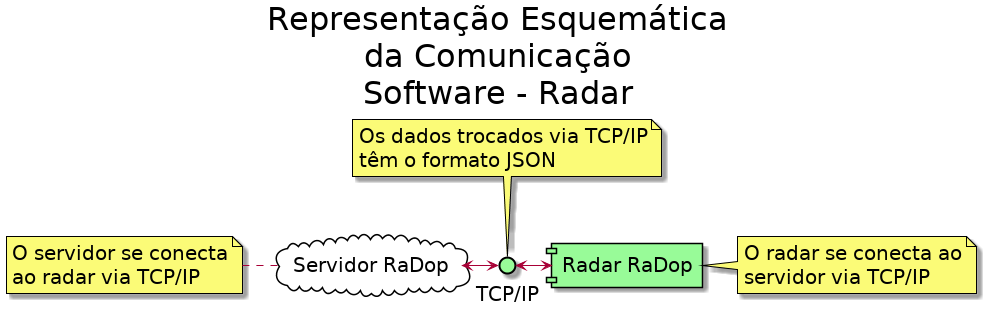
\includegraphics[width=\textwidth]{diagrama-comunicacao-software-radar.png}}
	\caption{\label{fig:diagrama-com-soft-radar} Diagrama que mostra como será a comunicação entre o servidor RaDop e o radar.}
\end{figure}

A comunicação será feita entre o servidor do RaDop e o Radar via protocolo TCP/IP. Ambos terão um endereço IP pelo do qual serão acessados. Esses endereços terão um único \textit{endpoint} para ser acessado nas comunicações, independente do tipo de dado enviado.

Como haverá um único \textit{endpoint} de ambos os lados, a diferenciação do tipo de comunicação sendo realizada será feita por intermédio do JSON enviado. Nele, haverá um atributo denominado "tipo", e através dele será determinado sobre qual tipo de comunicação aquele dado se trata.

Por fim, para confirmar o recebimento de um pacote, o recebedor deverá mandar uma resposta que irá atestar que o dado foi recebido.

\section{Banco de Dados}

Os produtos de software desenvolvidos pela equipe terão os seus dados divididos em dois bancos de dados, devido ao formato da construção de alguns sistemas.

Os sistemas de microsserviços trabalham de forma descentralizada e, em sua maioria, trabalharão com objetos JSON. Devido a este formato de trabalho, o banco de dados escolhido foi o \textit{RethinkDB}. Ele é um banco de dados \textit{NoSQL} de chave e valor, muito parecido com a natureza descritiva do JSON. Por consequência, a aplicação RaDop -- que estará fortemente apoiada nos microsserviços -- fará uso do mesmo banco de dados mas em um domínio próprio para os seus dados.

O sistema do \textit{Dashboard}, devido ao estilo arquitetural MVT (\textit{Model}, \textit{View} e \textit{Template}) e o mapeamento objeto-relacional, ORM (\textit{Object-Relational Mapping}), do \textit{Django}, a aplicação trabalha melhor com bancos de dados relacionais. Por isso, a equipe optou por usar um banco de dado relacional SQL, o \textit{PostgreSQL}. Ele fará parte do \textit{stack} de serviços que darão apoio ao \textit{Dashboard}.

A partir dessa escolha a equipe elaborou, com base nos requisitos e necessidades até aqui levantados, um modelo de classe que englobe os dois bancos de dados, que está melhor descrito na subseção abaixo.

\subsection{Diagrama de Classes}

A equipe de software do RaDop construiu a figura \ref{fig:diagrama-classe-soft} para tentar representar melhor como será o modelo de dados/objetos das aplicações de software. Devido ao fato que grande parte dos sistemas trabalham com tecnologias de JSON para o armazenamento de objetos, as classes derivaram destes arquivos definidos durante a execução dos sistemas.

JSON é um acrônimo de \textit{JavaScript Object Notation}, é um formato compacto, de padrão aberto independente, de troca de dados simples e rápida (\textit{parsing}) entre sistemas, especificado por Douglas Crockford em 2000, que utiliza texto legível a humanos, no formato atributo-valor (natureza auto-descritiva)\footnote{\cite{jsonorg}}.

A partir disso a equipe elaborou de uma forma simples e explicativa como se dariam as classes de objetos e suas relações por meio da representação em UML. Lembrando que novas classes e relacionamentos podem ser criados.

As classes representadas como \textit{Response} e \textit{Package} serão as classes representativas dos objetos de mensagem que serão trocados entre o Radar e o servidor de microsserviços, e posteriormente às aplicações.

\section{Resiliência na Comunicação do Software}

A comunicação dos diversos softwares entre si e com o radar são essenciais para o funcionamento do sistema neste projeto. Por isso, deve-se tornar o sistema criado o mais resiliente possível com relação à problemas de comunicação, para que o impacto desses seja o menor possível, caso ocorreram.

Por isso, foram levantados os principais problemas de comunicação entre os softwares ou destes com o radar, que poderão ocorrer dentro do escopo do presente projeto. A partir disso, foi-se definido que tipo de mecanismos estarão presentes para mitigar os efeitos dessas falhas para o funcionamento do sistema como um todo.

Abaixo estão listadas as falhas possíveis de ocorrerem, assim como as medidas para mitigar os efeitos delas:

\subsection{Impossibilidade de comunicação entre o radar e o sistema remoto}

\begin{itemize}
    \item \textbf{Descrição da falha:}

    A comunicação entre o radar e o sistema remoto é interrompida, impossibilitando a troca de dados entre ambos.

    \item \textbf{Mecanismo para mitigar a falha:}

    Os dados que não puderem ser enviados serão armazenados localmente (no radar e no serviço remoto) e transmitidos assim que a comunicação for restabelecida. Isso fará com que dados não deixem de ser enviados em caso de falha de comunicação.
\end{itemize}

\subsection{Impossibilidade de comunicação com algum microsserviço}

\begin{itemize}
    \item \textbf{Descrição da falha:}

     O envio ou recebimento de dados de um microsserviço é impossibilitado.

    \item \textbf{Mecanismo para mitigar a falha:}

    Toda nova requisição, independente se o serviço está ou não sem comunicação, será colocada em uma fila de execução. Esta fila permitirá com que o microsserviço não deixe de executar uma requisição em virtude de ter ficado sem comunicação.

    Além disso, o uso da fila proporcionará uma organização na ordem de execução dos pedidos. A ferramenta que será utilizada para gerenciar essas filas será o \textit{RabbitMQ}.
\end{itemize}

\subsection{Queda de um microsserviço}

\begin{itemize}
    \item \textbf{Descrição da falha:}

    Um microsserviço se torna indisponível, entendendo indisponibilidade como ele travar ou ser encerrado.

    \item \textbf{Mecanismo para mitigar a falha:}

    Os microsserviços serão colocados em contêineres da tecnologia \textit{Docker}. Isso permitirá que novas instâncias de microsserviços indisponíveis sejam criadas rapidamente, fazendo com que o tempo indisponível deles seja reduzido.

    Além disso, o uso dos contêineres permitirá que várias instâncias idênticas de um microsserviço estejam em funcionamento ao mesmo tempo e sejam criadas ou removidas a qualquer momento. Desse modo, será possível ter uma alta disponibilidade dos microsserviços, assim como escalabilidade.
\end{itemize}

\section{\textit{DevOps}}

\textit{DevOps} é um termo criado a partir da união de dois termos, o \textit{Dev} é atribuido ao \textit{development}, ou seja, a parte de desenvolvimento da organização. Já o \textit{Ops} diz respeito à \textit{operations}, o setor da organização relacionado à operações. O \textit{DevOps} descreve um conjunto de práticas para integração entre os setores de desenvolvimento, operações, além da adoção de processos automatizados para produção rápida e segura de aplicações e serviços. É um processo que é factível o desenvolvimento ágil de aplicações.

Segundo Ebert \cite{ebert2016devops} o \textit{DevOps} trata de processos de negócios de desenvolvimento e provisionamento rápidos e flexíveis. Integra de forma eficiente o desenvolvimento, a entrega e as operações, facilitando assim uma conexão enxuta e fluida desses silos tradicionalmente separados.

Dentro do projeto RaDop, a equipe de software buscará seguir algumas das melhores práticas do processo para garantir agilidade e segurança durante o desenvolvimento dos produtos. As práticas implementadas serão:
\begin{itemize}
    \item Integração Contínua (CI): Para garantir a qualidade e a uniformidade de todo o código novo que entra no sistema, os produtos de softwares estarão inseridos num \textit{pipeline}, onde passarão por testes de padrão de desenvolvimento, testes de código, testes estáticos, testes de segurança e testes de construção de serviços. Com a execução exitosa de todos os testes nos novos serviços, assim como nas evoluções dos antigos, estes serão integrados com as versões anteriores e os demais serviços.
    \item Entrega Contínua (CD): Com a garantia de que as novas versões, e evoluções, estão de acordo com o planejado, esses novos produtos, ou subprodutos, serão entregues e implementados no seu destino (serviço do servidor, aplicativo ou \textit{Dashboard}) mais rapidamente e estarão prontamente disponíveis para uso.
    \item \textit{Docker}: Para provisionamento dos serviços, implantação e isolamento dos ambientes e requerimentos. Além de auxiliar na escalabilidde dos serviços e possibilitar ações ágeis sobre erros e dificuldades.
\end{itemize}

\section{Protótipos}

Todas as telas referentes à construção da interface entre o sistema e o usuário foram desenhadas para auxiliar o time na construção do software e pensando também na melhor usabilidade para o usuário.

Segue abaixo as telas da interface do aplicativo e do \textit{dashboard} do RaDop.

\begin{figure}[ht]
	\center{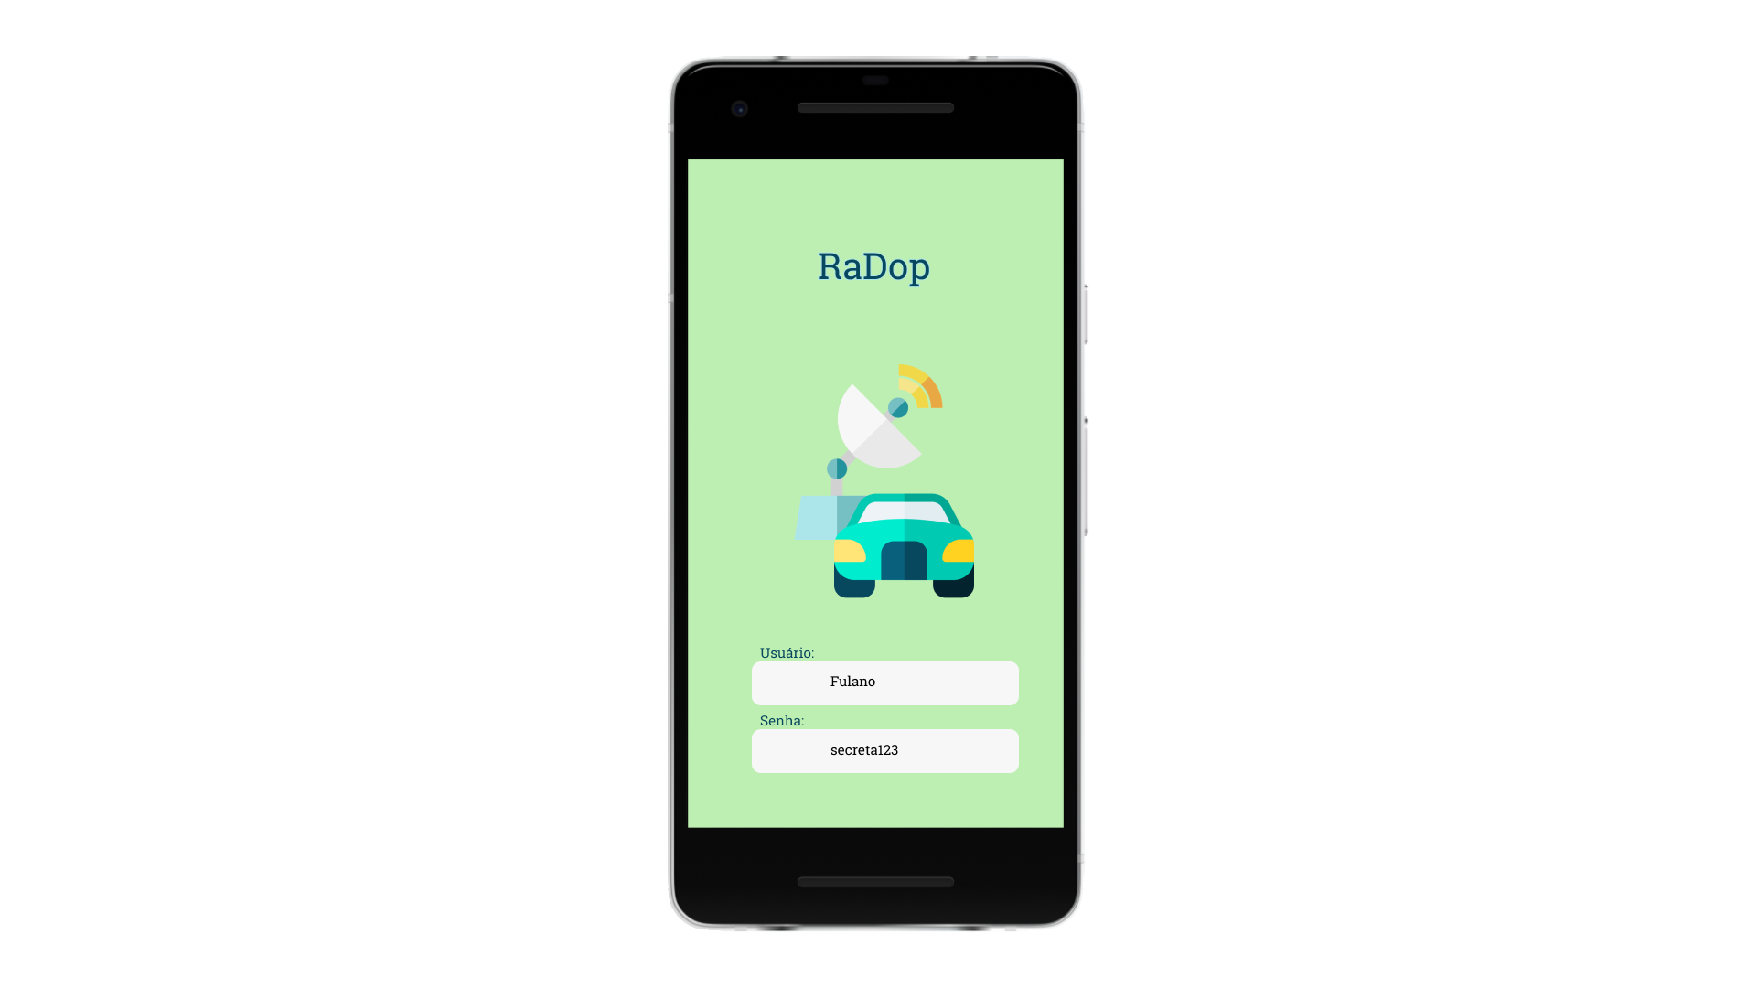
\includegraphics[scale=0.5]{tela_inicial_aplicativo.pdf}}
	\caption{\label{fig:tela_inicial} Protótipo da tela inicial do aplicativo RaDop.}
\end{figure}\newpage

\begin{figure}[ht]
	\center{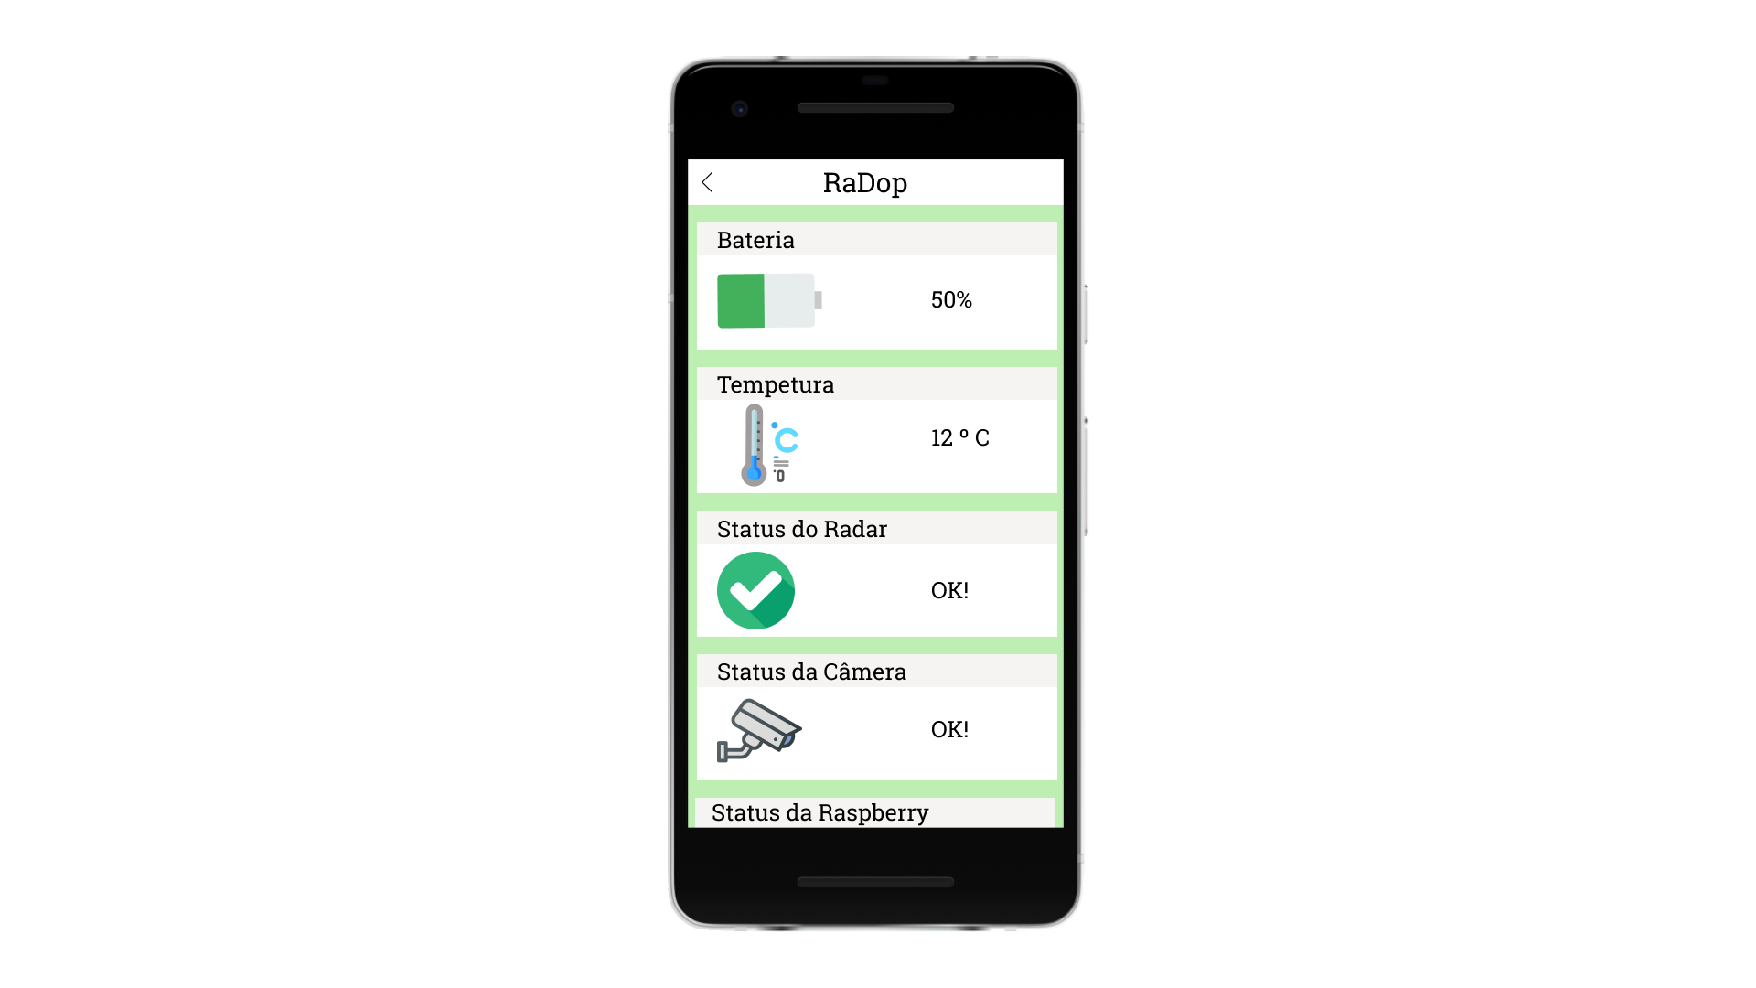
\includegraphics[scale=0.5]{tela_status.pdf}}
	\caption{\label{fig:tela_status} Protótipo da tela com os estados de funcionamento do radar.}
\end{figure}\newpage

\begin{figure}[ht]
	\center{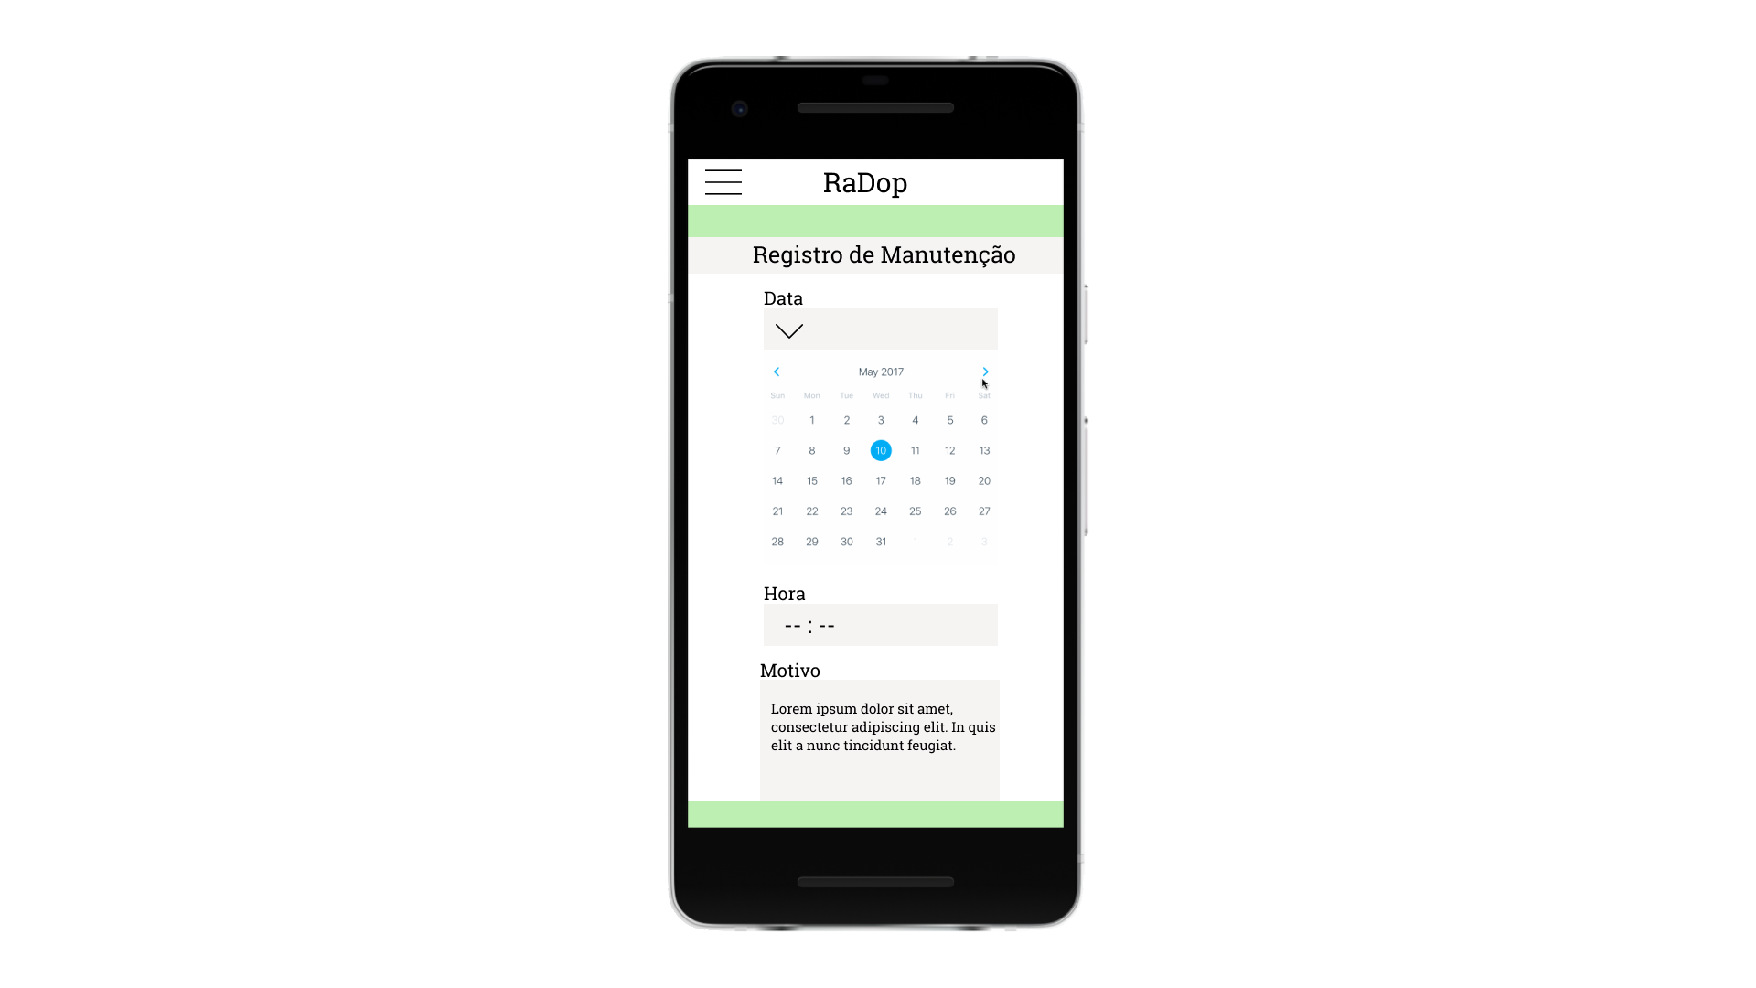
\includegraphics[scale=0.5]{tela_registro.pdf}}
	\caption{\label{fig:tela_registro} Protótipo da tela de registro para o usuário administrador poder cadastrar a manutenção do radar.}
\end{figure}\newpage

\begin{figure}[ht]
	\center{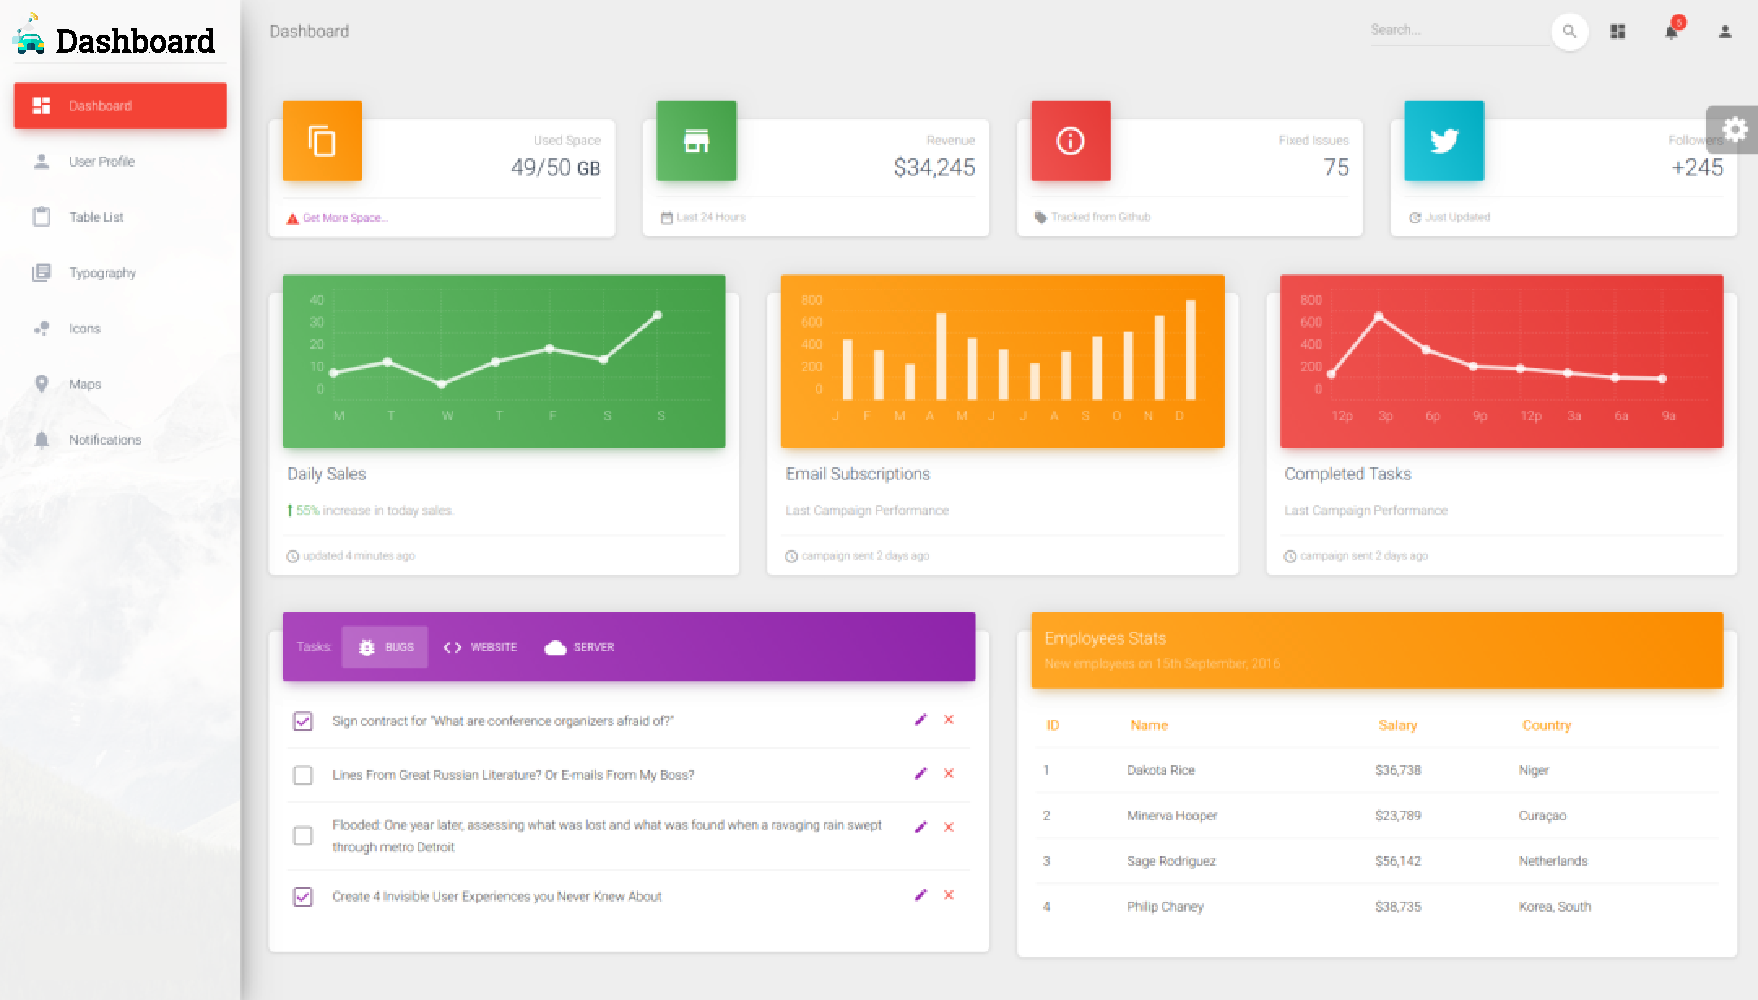
\includegraphics[scale=0.5]{tela_dashboard.pdf}}
	\caption{\label{fig:tela_dashboard} Protótipo da tela principal do dashboard do radar.}
\end{figure}\newpage

\chapter{Apêndices}
\begin{figure}[h!]
	\center{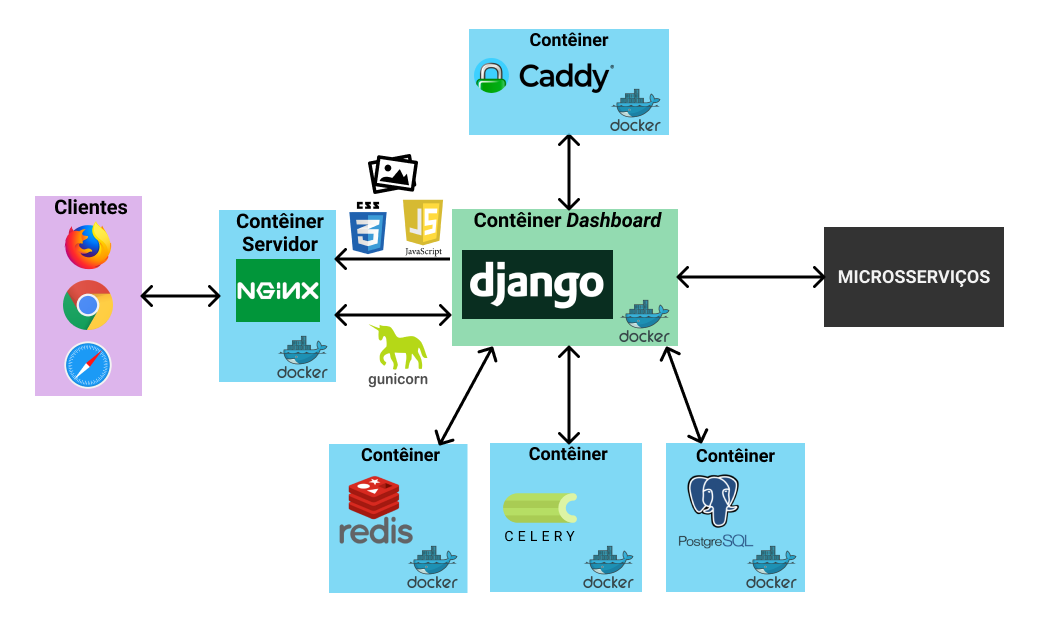
\includegraphics[width=\textwidth]{diagrama-arq-dashboard.png}}
	\caption{\label{fig:diagrama-arq-dashboard} Diagrama que mostra a arquitetura e tecnologias que serão usadas com o \textit{Dashboard}.}
\end{figure}

\begin{figure}[h!]
	\center{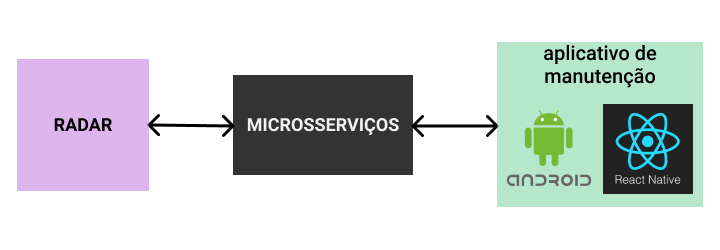
\includegraphics[width=\textwidth]{diagrama-arq-webApp.png}}
	\caption{\label{fig:diagrama-arq-webApp} Diagrama que mostra a arquitetura e tecnologias que serão usadas com o \textit{WebApp}.}
\end{figure}

\begin{figure}[!h]
	\center{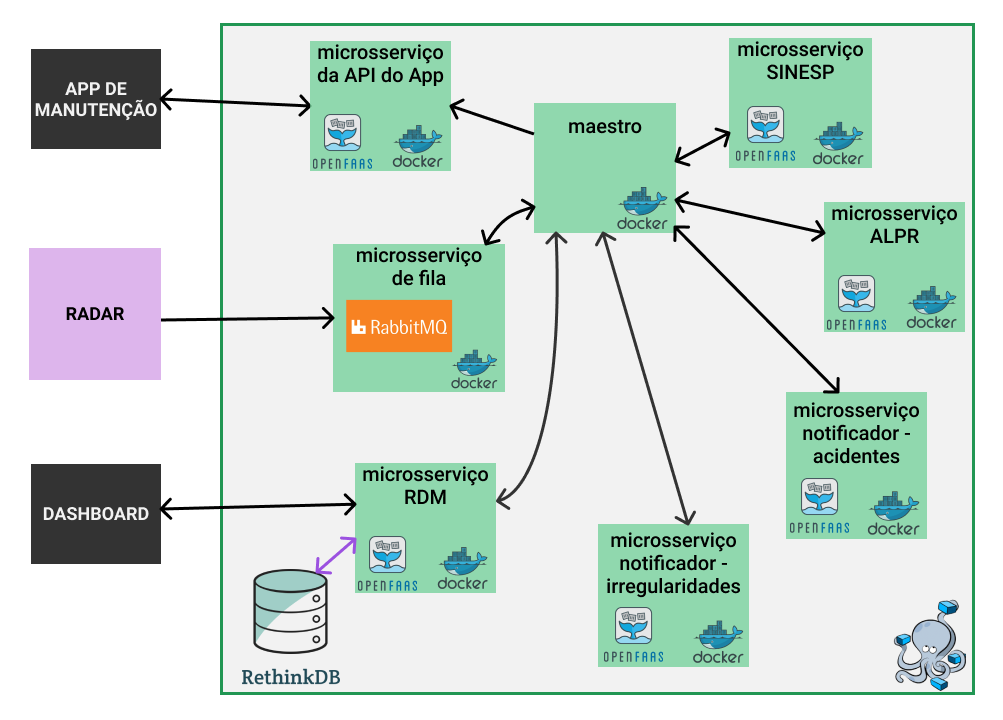
\includegraphics[width=\textwidth]{diagrama-arq-microsservicos.png}}
	\caption{\label{fig:diagrama-arq-microsservicos} Diagrama que mostra a arquitetura e tecnologias que serão usadas com os microsserviços.}
\end{figure}

\begin{figure}[ht]
	\center{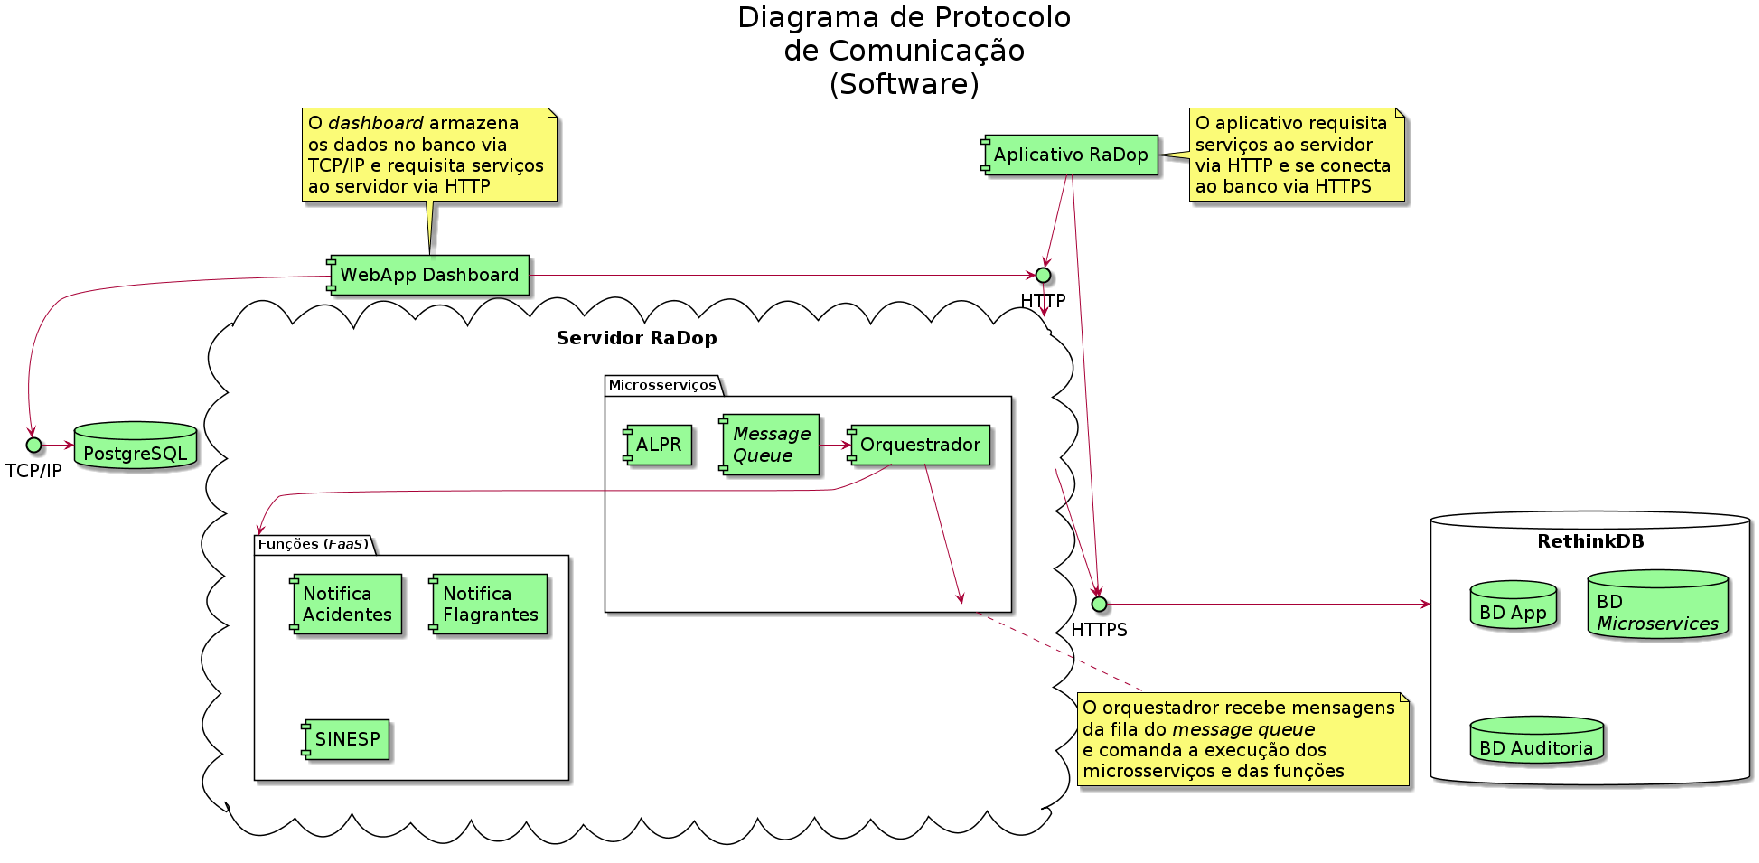
\includegraphics[scale=0.5]{diagrama-de-comunicacao-PC2.pdf}}
	\caption{\label{fig:diagrama-comm-soft} Diagrama de comunicação dos serviços de software.}
\end{figure}

\begin{figure}[ht]
	\center{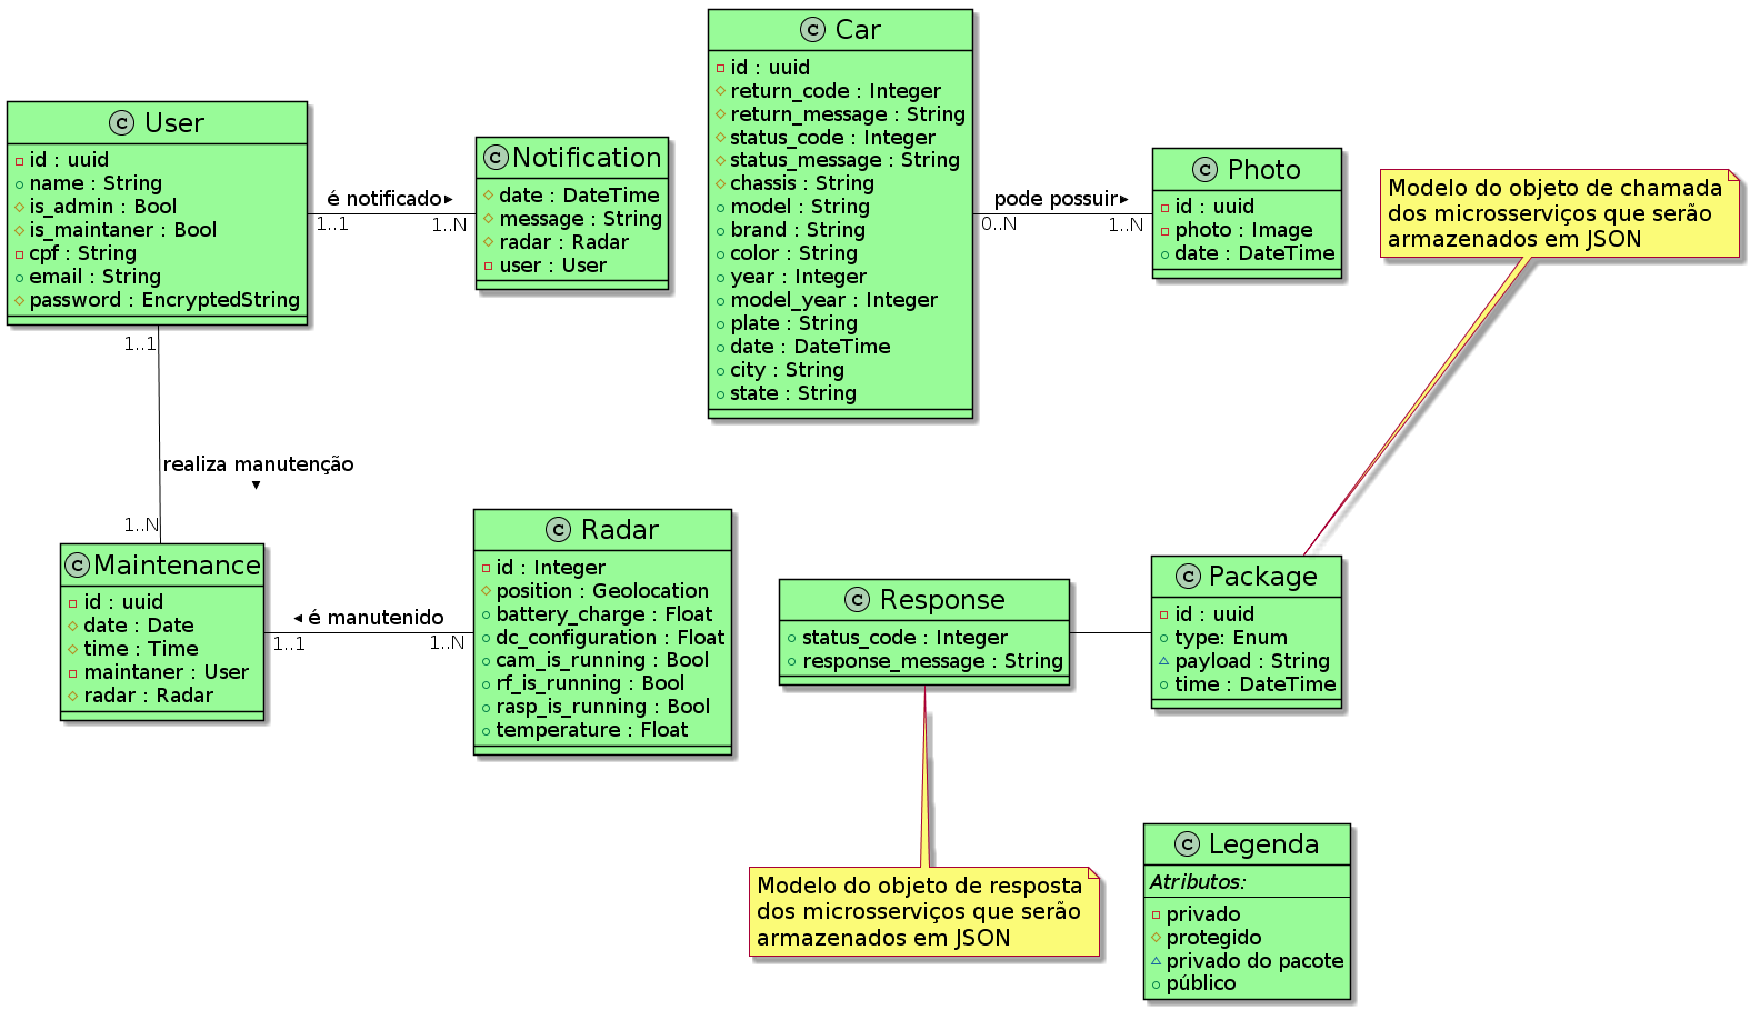
\includegraphics[scale=0.5]{diagrama-de-classes-PC2.pdf}}
	\caption{\label{fig:diagrama-classe-soft} Diagrama UML de classes dos produtos de software.}
\end{figure}
